% gc-06-ChainRule.tex

\documentclass[xcolor=dvipsnames]{beamer}

\usepackage{cancel}
\renewcommand{\CancelColor}{\color{red}}
\usepackage{graphicx}
\usepackage{wrapfig}
\usepackage{colortbl}
\definecolor{myblue}{rgb}{0.8,0.85,1}

\mode<presentation>
{
  \usetheme{Warsaw}
  \setbeamercovered{transparent}
}
% \usecolortheme[named=OliveGreen]{structure}
\setbeamertemplate{navigation symbols}{} 
\setbeamertemplate{blocks}[rounded][shadow=true] 

\newif\ifBCITCourse
\BCITCoursetrue
% \BCITCoursefalse
\newif\ifWhichCourse
\WhichCoursetrue
\WhichCoursefalse
\ifBCITCourse
\ifWhichCourse
\newcommand{\CourseName}{Statistics for Food Technology}
\newcommand{\CourseNumber}{MATH 2441}
\newcommand{\CourseInst}{BCIT}
\else
\newcommand{\CourseName}{Calculus for Geomatics}
\newcommand{\CourseNumber}{MATH 2511}
\newcommand{\CourseInst}{BCIT}
\fi
\else
\newcommand{\CourseName}{Philosophy and Literature}
\newcommand{\CourseNumber}{PHIL 375}
\newcommand{\CourseInst}{UBC}
\fi

\title{Chain Rule}
\subtitle{{\CourseNumber}, BCIT}

\author{\CourseName}

\date{January 23, 2017}

% \begin{figure}[h]
% 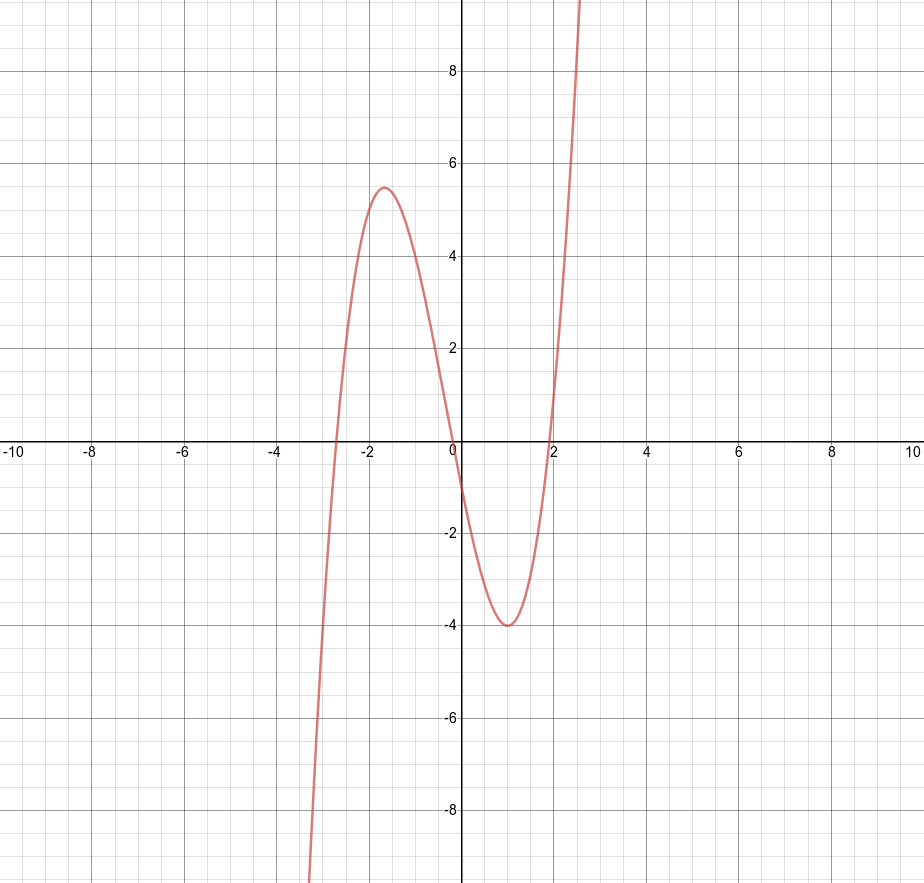
\includegraphics[scale=.3]{./diagrams/extrema1.png}
% \end{figure}

\begin{document}

\begin{frame}
  \titlepage
\end{frame}

\begin{frame}
  \frametitle{Euler's Number}
The number $e$ is defined as follows,
\begin{equation}
  \label{eq:ciedaeme}
  e=\lim_{t\rightarrow\infty}\left(1+\frac{1}{t}\right)^{t}
\end{equation}
\end{frame}

\begin{frame}
  \frametitle{Lemma}
Consider two functions $f_{1}$ and $f_{2}$. They are related in so far
as
\begin{equation}
  \label{eq:ohquailo}
  f_{1}(x)=f_{2}\left(\frac{1}{x}\right)
\end{equation}
For example,
\begin{equation}
  \label{eq:seemaxah}
  f_{1}(x)=\frac{2x+1}{5x-7}\mbox{ and }f_{2}(x)=-\frac{x+2}{7x-5}
\end{equation}
Then
\begin{equation}
  \label{eq:iebieluk}
  \mbox{If }\lim_{x\rightarrow\infty}f_{1}(x)=a\mbox{ then }\lim_{x\rightarrow{}0}f_{2}(x)=a
\end{equation}
% The derivative of $f(x)=\ln{}x$ is
% \begin{equation}
%   \label{eq:ailiebai}
%   f'(x)=\frac{1}{x}
% \end{equation}
% We will not give a proof for the derivative of the exponential
% function. The derivative of the logarithmic function follows from the
% derivative of the exponential function and the chain rule. To show how
% this works we need to learn the chain rule.
\end{frame}

\begin{frame}
  \frametitle{The Derivative of the Logarithmic Function}
Now consider the function $f(x)=\ln{}x$ and the definition of the
derivative,
\begin{equation}
  \label{eq:eeghaphe}
  f'(x)=\lim_{h\rightarrow{}0}\frac{f(x+h)-f(x)}{h}=\lim_{h\rightarrow{}0}\frac{1}{h}\ln\frac{x+h}{x}=\notag
\end{equation}
\begin{equation}
  \label{eq:quanoefe}
  \lim_{h\rightarrow{}0}\frac{1}{x}\cdot\frac{x}{h}\ln\left(1+\frac{h}{x}\right)=\lim_{h\rightarrow{}0}\frac{1}{x}\ln\left(1+\frac{1}{\frac{x}{h}}\right)^{\frac{x}{h}}
\end{equation}
Use the lemma of the last slide and the definition of Euler's number to see that
\begin{equation}
  \label{eq:oozeexei}
  f'(x)=\frac{1}{x}
\end{equation}
\end{frame}

\begin{frame}
  \frametitle{Problematic Functions}
Here are some functions that we either don't know how to differentiate
or whose differentiation would take an inordinate amount of time.
\begin{equation}
  \label{eq:faegeehi}
f(x)=2^{x}
\end{equation}
\begin{equation}
  \label{eq:kooteiju}
f(x)=\sqrt{x^{2}+1}
\end{equation}
\begin{equation}
  \label{eq:oochahph}
f(x)=(x^{2}+x+1)^{100}
\end{equation}
\begin{equation}
  \label{eq:bongaeza}
f(x)=\sin(1+\sqrt{x-7})
\end{equation}
\begin{equation}
  \label{eq:ooquonge}
f(x)=\log_{10}x
\end{equation}
\begin{equation}
  \label{eq:iejafaic}
f(x)=\ln(x^{2}+1)
\end{equation}
\end{frame}

\begin{frame}
  \frametitle{The Chain Rule}
  \begin{block}{Rule 7}
The Chain Rule
  \end{block}
\begin{equation}
  \label{eq:aepuaxai}
g'(x)=f_{1}'(f_{2}(x))f_{2}'(x)\mbox{ for }g(x)=(f_{1}\circ{}f_{2})(x)
\end{equation}
\end{frame}

\begin{frame}
  \frametitle{Chain Rule Reason}
Consider
\begin{align}
  \label{eq:prf}
  (f\circ{}g)'(x)=\lim_{h\rightarrow{}0}\frac{f(g(x+h))-f(g(x))}{h}&=&\notag \\
  \lim_{h\rightarrow{}0}\frac{f(g(x+h))-f(g(x))}{g(x+h)-g(x)}\cdot\lim_{h\rightarrow{}0}\frac{g(x+h)-g(x)}{h}&=& \\
  f'(g(x))g'(x)&&
\end{align}
This is only a hint, not a rigorous proof, since we have replaced
$g(x+h)$ by $g(x)+h$, which isn't covered by our rules and is, in
fact, false in some situations.
\end{frame}

\begin{frame}
  \frametitle{Exercises}
  \begin{enumerate}
  \item<1-> Diffentiate: $f(x)=2^{x}$
  \item<2-> Diffentiate: $f(x)=\sqrt{x^{2}+1}$
  \item<3-> Diffentiate: $f(x)=(x^{2}+x+1)^{100}$
  \item<4-> Diffentiate: $f(x)=\log_{10}x$
  \item<5-> Diffentiate: $f(x)=\ln(x^{2}+1)$
  \end{enumerate}
\end{frame}

\begin{frame}
  \frametitle{Inverse and Identity Function}
Remember how we defined the logarithmic function,
\begin{equation}
  \label{eq:tieteiph}
  \ln{}y=x\mbox{ if and only if }e^{x}=y
\end{equation}
so the logarithmic function is the inverse of the exponential
function. Consequently, if $f(x)=e^{x}$ and $g(y)=\ln{}y$
\begin{equation}
  \label{eq:iewaebef}
  (f\circ{}g)(y)=y\mbox{ and }(g\circ{}f)(x)=x
\end{equation}
When (\ref{eq:iewaebef}) is true we call $f$ the \alert{inverse
  function} of $g$ and vice versa. The function $\mbox{id}(x)=x$ is called
the \alert{identity function}. 
\end{frame}

\begin{frame}
  \frametitle{The Derivative of the Exponential Function}
We know the derivative of the identity function.
\begin{equation}
  \label{eq:sivahzuw}
  \mbox{id}'(x)=1
\end{equation}
Consequently,
\begin{equation}
  \label{eq:zeejaixu}
  \frac{d}{dx}\ln\left(e^{x}\right)=1
\end{equation}
We also know that according to the chain rule
\begin{equation}
  \label{eq:iecheixo}
  \frac{d}{dx}\ln\left(e^{x}\right)=\frac{1}{e^{x}}\exp'(x)
\end{equation}
where $\exp(x)=e^{x}$. Therefore,
\begin{equation}
  \label{eq:zigaewai}
  \exp'(x)=e^{x}
\end{equation}
The exponential function is its own derivative!
\end{frame}

\begin{frame}
  \frametitle{Derivative of the Exponential Function: Exercises}
Differentiate the following functions:
\begin{equation}
  \label{eq:beetulae}
f(x)=e^{\sin{}x}  
\end{equation}
\begin{equation}
  \label{eq:aekephii}
g(t)=\frac{1}{e^{t}}  
\end{equation}

\bigskip

\begin{equation}
  \label{eq:uijeabai}
v(w)=w^{2}e^{w}  
\end{equation}

\bigskip

\begin{equation}
  \label{eq:ohzabeed}
g(z)=\frac{e^{z}-1}{e^{z}+1}  
\end{equation}
\end{frame}

\begin{frame}
  \frametitle{Exercises for Differentiation I}
Differentiate the following functions or find $dy/dx$ for the
following curves:
\begin{equation}
  \label{eq:pimexeiz}
  f(\vartheta)=\tan(\sin{}\vartheta)
\end{equation}
\begin{equation}
  \label{eq:oogheica}
  F(x)=\sqrt[4]{1+2x+x^{3}}
\end{equation}
\begin{equation}
  \label{eq:ibagheab}
  g(t)=\frac{\pi}{(t^{4}+1)^{3}}
\end{equation}
\begin{equation}
  \label{eq:oboohoca}
  f(s)=\sqrt[3]{1+\tan{}s}
\end{equation}
\begin{equation}
  \label{eq:choopaib}
  y=(x^{2}+1)\sqrt[3]{x^{2}+2}
\end{equation}
\begin{equation}
  \label{eq:uosiamei}
y=e^{x\cos{}x}  
\end{equation}
\begin{equation}
  \label{eq:oshaiphu}
  y=x\sin\frac{1}{x}
\end{equation}
\end{frame}

\begin{frame}
  \frametitle{Exercises for Differentiation II}
Differentiate the following functions or find $dy/dx$ for the
following curves:
\begin{equation}
  \label{eq:ciukaech}
  y=3\cot(nx)
\end{equation}
\begin{equation}
  \label{eq:oveagooy}
  y=xe^{-kx}
\end{equation}
\begin{equation}
  \label{eq:veeveema}
  h(t)=(t^{4}-1)^{3}(t^{3}+1)^{4}
\end{equation}
\begin{equation}
  \label{eq:athaazui}
  y=(x^{2}+1)\sqrt{x^{2}+2}
\end{equation}
\begin{equation}
  \label{eq:ahgoovim}
  G(y)=\left(\frac{y^{2}}{y+1}\right)^{5}
\end{equation}
\begin{equation}
  \label{eq:gaidaime}
  y=\tan^{2}(3\vartheta)
\end{equation}
\end{frame}

\begin{frame}
  \frametitle{Exercises for Differentiation III}
Find an equation of the tangent line to the curve
\begin{equation}
  \label{eq:vaixohga}
  y=\frac{2}{1+e^{-x}}
\end{equation}
at $x=0$.

\bigskip

Here is a model for the length of daylight (in hours) in Toronto on
the $t$-th day of the year
\begin{equation}
  \label{eq:iefeuvae}
  L(t)=12+2.8\sin\left(\frac{2\pi}{365}(t-80)\right)
\end{equation}
Compare how the number of hours of daylight is increasing in Toronto
on March 21 and May 21.
\end{frame}

\begin{frame}
  \frametitle{End of Lesson}
Next Lesson: Higher Order Derivatives
\end{frame}

\end{document}
